\section{介绍}

%------------------------------------------------
\begin{frame}[fragile]{Our Design}
我们BAN 的原本设计是这样的:
\begin{figure}[htbp]
\begin{center}
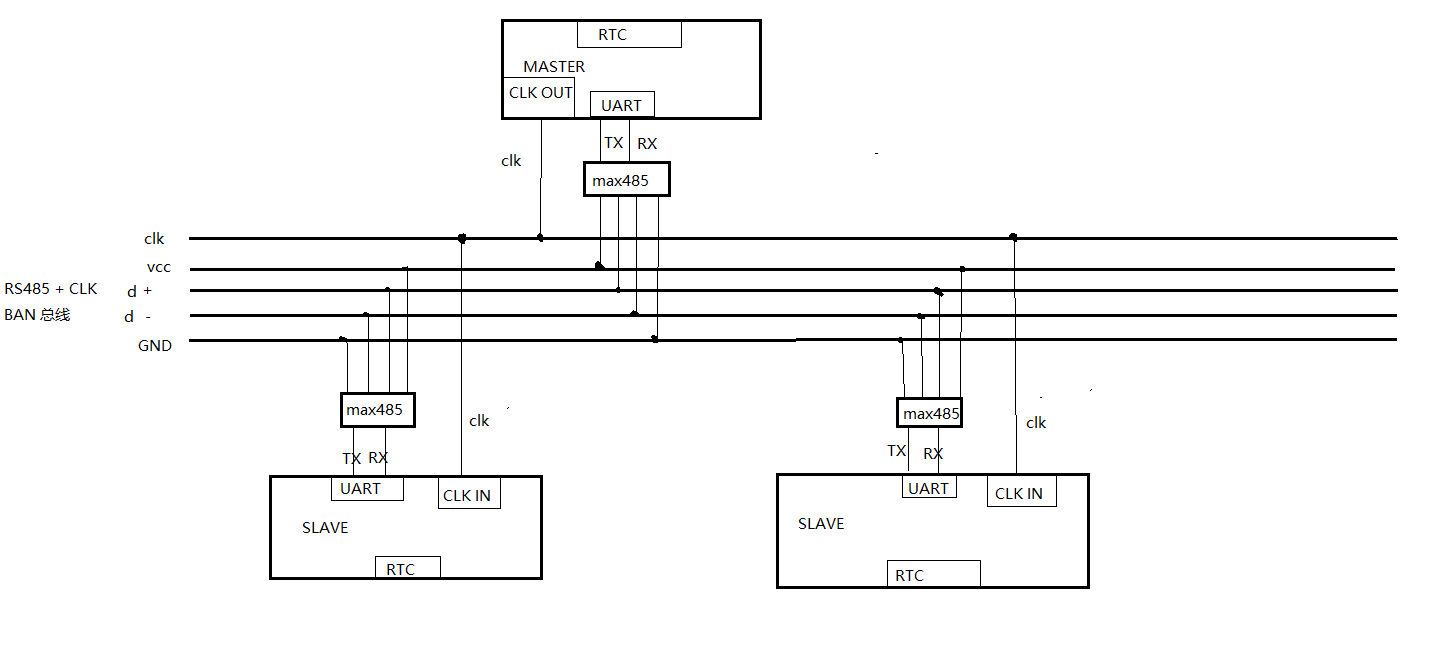
\includegraphics[width=10cm]{img/overview}
\caption{BAN }
\label{Overview}
\end{center}
\vspace{-0.5em}
\end{figure}
\end{frame}


%------------------------------------------------
\begin{frame}[fragile]{BUS}
1. 由 RS485 增添一根 clk线 形成 BAN 总线的 基本硬件线路。

2. clk 用于产生 ms 级别的脉冲波,用于时钟的同步。

3.  d+ d- 是差分处理后的数据信号。

图\ref{Overview} 假设了 挂载在总线上的设备有一个主机,两个从机。

\end{frame}

%------------------------------------------------
\begin{frame}[fragile]{UART \& 485}

max485 是一型 RS232 转 RS485 的芯片,可以把串口数据 转化为 差分信号,使其符合\textbf{RS-485}
电气规范。

STM32 方面需要实现串口的驱动,使确保串口可以实时的发送数据。接收数据。

\end{frame}

%------------------------------------------------
\begin{frame}[fragile]{RTC \& CLK}
本地时钟用于本地计数,同步时钟用于同步BAN 上设备的时钟。
\begin{itemize}
\item  RTC ,本地时钟。 每个设备都有个本地时钟。 计时粒度为 100us.

\item  CLK,同步时钟。 BAN总线上的设备使用时钟线来完成时钟同步。主设备的定时器产生同步脉冲,从设备
的定时器捕获同步脉冲完成同步。
\end{itemize}


\end{frame}


%------------------------------------------------
\begin{frame}[fragile]{Demo}

在demo 中,为了克服硬件条件的限制,我们:
\begin{itemize}
    \item 没有使用max485 来完成\textbf{TTL信号}转\textbf{差分信号}.
    \item 使用另外的一个定时器来模拟RTC的功能。
    \item 只能模拟一个主设备,一个从设备的情况。
    \item 使用串口
\end{itemize}

\end{frame}


%------------------------------------------------
\begin{frame}[fragile]{Demo 连线}

下图是demo 的连线和结构图:
\begin{figure}[htbp]
\begin{center}
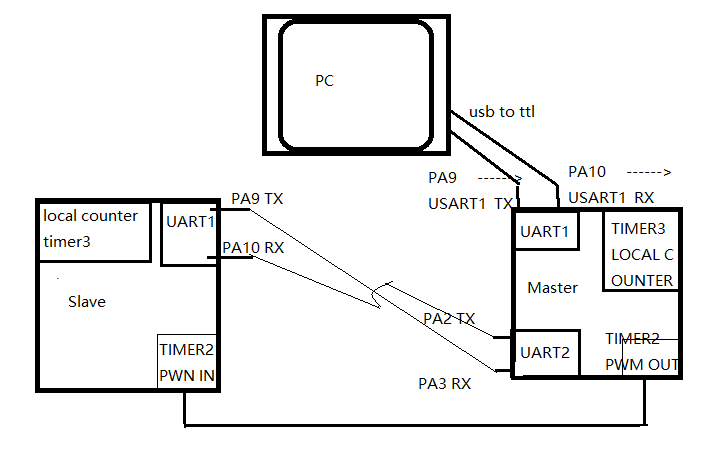
\includegraphics[width=10cm]{img/demo0}
\caption{demo}
\label{Overview}
\end{center}
\vspace{-0.5em}
\end{figure}

\end{frame}
